\documentclass[tikz]{standalone}
\usepackage{amsmath}
\usepackage{tikz}

\begin{document}

\begin{figure}[h]
\begin{center}
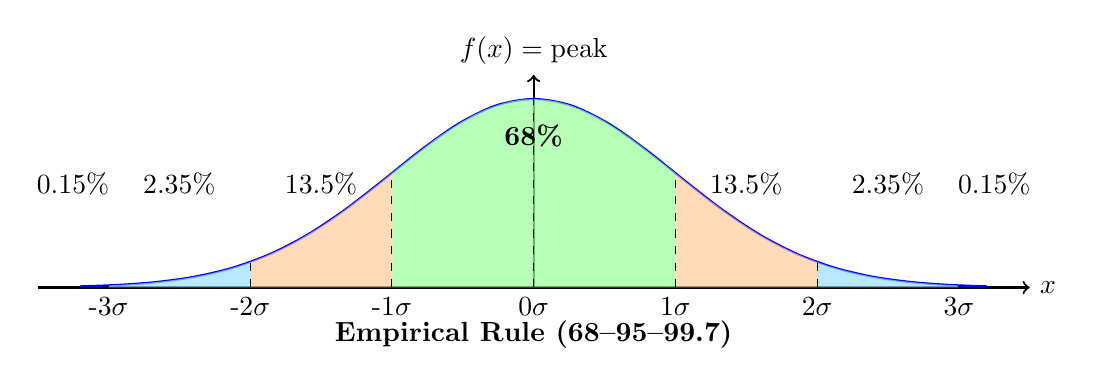
\begin{tikzpicture}[xscale=1.8, yscale=6]
  \draw[->, thick] (-3.5,0) -- (3.5,0) node[right] {$x$};
  \draw[->, thick] (0,0) -- (0,0.45) node[above] {$f(x) = \text{peak}$};

  \draw[domain=-3.2:3.2, smooth, variable=\x, thick, blue] 
    plot ({\x}, {1/sqrt(2*pi) * exp(-0.5*\x*\x)});

  \fill[green!40, opacity=0.7] 
    plot[domain=-1:1] (\x, {1/sqrt(2*pi) * exp(-0.5*\x*\x)}) -- (1,0) -- (-1,0) -- cycle;

  \fill[orange!40, opacity=0.7] 
    plot[domain=-2:-1] (\x, {1/sqrt(2*pi) * exp(-0.5*\x*\x)}) -- (-1,0) -- (-2,0) -- cycle;
  \fill[orange!40, opacity=0.7] 
    plot[domain=1:2] (\x, {1/sqrt(2*pi) * exp(-0.5*\x*\x)}) -- (2,0) -- (1,0) -- cycle;

  \fill[cyan!40, opacity=0.7] 
    plot[domain=-3:-2] (\x, {1/sqrt(2*pi) * exp(-0.5*\x*\x)}) -- (-2,0) -- (-3,0) -- cycle;
  \fill[cyan!40, opacity=0.7] 
    plot[domain=2:3] (\x, {1/sqrt(2*pi) * exp(-0.5*\x*\x)}) -- (3,0) -- (2,0) -- cycle;

  \foreach \x in {-3,-2,-1,0,1,2,3} {
    \draw[dashed] (\x,0) -- (\x,{1/sqrt(2*pi) * exp(-0.5*\x*\x)});
    \node[below] at (\x,0) {\x$\sigma$};
  }

  \node at (0,0.32) {\textbf{68\%}};
  \node at (-1.5,0.22) {13.5\%};
  \node at (1.5,0.22) {13.5\%};
  \node at (-2.5,0.22) {2.35\%};
  \node at (2.5,0.22) {2.35\%};
  \node at (-3.25,0.22) {0.15\%};
  \node at (3.25,0.22) {0.15\%};

  \node[font=\bfseries] at (0,-0.1) {Empirical Rule (68–95–99.7)};
\end{tikzpicture}
\end{center}
\caption{An illustration of the empirical rule.}
\end{figure}

\end{document}